\chapter{Pengenalan Machine Learning: Supervised Learning}

\section{Peran Machine Learning dalam Era Big Data}

Perkembangan teknologi dan meningkatnya kemampuan organisasi dalam mengumpulkan serta menyimpan data dalam jumlah besar telah mendorong lahirnya era Big Data. Karakteristik Big Data yang dikenal dengan 5V — volume, velocity, variety, veracity, dan value — menggambarkan kompleksitas sekaligus potensi yang dapat dimanfaatkan untuk keunggulan kompetitif \cite{laney2001,gandomi2015,nist2015}.

Dalam konteks ini, \textbf{Machine Learning (ML)} menjadi komponen krusial dalam \textit{Big Data Value Chain}, khususnya pada tahapan analisis dan ekstraksi wawasan setelah proses integrasi dan penyimpanan data. ML memungkinkan organisasi untuk berpindah dari analisis deskriptif ke arah analisis prediktif dan preskriptif yang jauh lebih bernilai dalam pengambilan keputusan \cite{chen2012,wamba2017}.

Berbagai sektor bisnis telah menerapkan ML untuk berbagai keperluan, antara lain:
- Prediksi churn pelanggan di industri telekomunikasi dan ritel,
- Deteksi penipuan dalam sektor keuangan,
- Prediksi permintaan di rantai pasok,
- Rekomendasi produk di e-commerce \cite{mcafee2012,mariani2021,georgescu2020}.

Secara strategis, ML memperluas cakupan manfaat Big Data dari sekadar "pengetahuan tentang masa lalu" menjadi "pengetahuan tentang masa depan" melalui kemampuan prediksi berbasis pola data historis. Hal ini memungkinkan organisasi untuk membuat keputusan yang lebih cepat, tepat, dan terukur \cite{jeble2018,oecd2015,assuncao2015}.

Dalam konteks Big Data for Business, pemahaman dasar tentang ML, khususnya supervised learning, menjadi bekal penting bagi pengambil keputusan non-teknis agar dapat berkolaborasi secara efektif dengan tim data dan memanfaatkan hasil model secara optimal untuk kepentingan strategis organisasi \cite{provost2013data,fernandez2020,davenport2018}.



\section{Pengantar Machine Learning}

\textbf{Machine Learning (ML)} merupakan cabang dari kecerdasan buatan yang memungkinkan komputer belajar dari data tanpa perlu diprogram secara eksplisit untuk setiap aturan atau kondisi. Secara intuitif, ML bekerja dengan cara mengenali pola dalam data historis dan menggunakan pola tersebut untuk membuat prediksi atau keputusan terhadap data baru \cite{kelleher2015fundamentals}.

Dalam konteks analisis data bisnis, pendekatan konvensional (berbasis aturan) biasanya mengandalkan logika "jika–maka" yang ditentukan oleh pakar atau pengembang sistem. Sebagai contoh, dalam sistem deteksi penipuan berbasis aturan, programmer akan menetapkan aturan seperti: \textit{jika transaksi lebih dari 100 juta dan dilakukan di luar negeri, maka flag sebagai penipuan}. Meskipun efektif untuk skenario yang diketahui sebelumnya, pendekatan ini memiliki keterbatasan dalam skala besar, variasi tinggi, serta dinamika data yang terus berubah.

Sebaliknya, pendekatan Machine Learning memungkinkan sistem untuk secara otomatis membangun model dari data yang tersedia. Dengan menyediakan data historis yang telah diberi label (misalnya: transaksi yang diketahui sebagai penipuan atau bukan), algoritma ML akan mempelajari pola dan relasi antar variabel untuk kemudian digunakan pada data baru. Hal ini sangat berguna dalam menghadapi kompleksitas data bisnis modern yang tidak dapat ditangani hanya dengan aturan eksplisit.

ML juga bersifat adaptif. Model dapat diperbarui seiring waktu dengan data terbaru, sehingga tetap relevan dalam lingkungan bisnis yang dinamis. Contohnya, sistem rekomendasi produk pada platform e-commerce dapat belajar dari riwayat pembelian dan perilaku pengguna, kemudian menyesuaikan rekomendasi secara personalisasi.

Oleh karena itu, pemahaman terhadap prinsip dasar Machine Learning menjadi semakin penting bagi para pengambil keputusan di bidang bisnis dan manajemen, terutama dalam era Big Data yang menuntut kecepatan, akurasi, dan skalabilitas dalam pengambilan keputusan berbasis data.


\section{Tipe-Tipe Learning pada Machine Learning }

Machine Learning (ML) dapat diklasifikasikan ke dalam tiga tipe utama berdasarkan cara model belajar dari data, yaitu: \textbf{supervised learning}, \textbf{unsupervised learning}, dan \textbf{reinforcement learning} \cite{provost2013data}.

\textbf{1. Supervised Learning}  
Supervised learning adalah tipe machine learning di mana model belajar dari data yang sudah diberi label, artinya setiap data input (fitur) disertai dengan output yang benar (label). Tujuannya adalah agar model dapat mempelajari hubungan antara input dan output tersebut, sehingga dapat memprediksi output baru secara akurat.  
Contoh umum dalam bisnis meliputi:
- \textit{Prediksi churn pelanggan}: menggunakan riwayat transaksi dan interaksi pelanggan untuk memprediksi apakah pelanggan akan berhenti berlangganan.
- \textit{Estimasi penjualan}: memprediksi jumlah penjualan produk berdasarkan musim, lokasi, dan tren sebelumnya.
- \textit{Kredit scoring}: memprediksi risiko gagal bayar berdasarkan histori kredit dan data demografis.

Supervised learning merupakan pendekatan yang paling umum digunakan dalam aplikasi bisnis karena tersedia banyak data historis yang telah diberi label, dan hasil prediksinya mudah diinterpretasikan oleh pengambil keputusan \cite{chen2012,davenport2018}.

\textbf{2. Unsupervised Learning}  
Unsupervised learning digunakan ketika data tidak memiliki label. Tujuannya adalah menemukan struktur atau pola tersembunyi di dalam data.  
Contoh penerapannya dalam bisnis:
- \textit{Segmentasi pelanggan}: mengelompokkan pelanggan ke dalam segmen berdasarkan perilaku, preferensi, atau profil.
- \textit{Deteksi anomali}: menemukan transaksi mencurigakan tanpa diberi label penipuan secara eksplisit.

Teknik umum dalam unsupervised learning termasuk \textit{clustering} (misalnya k-means) dan \textit{dimensionality reduction} (misalnya PCA).

\textbf{3. Reinforcement Learning}  
Reinforcement learning adalah pendekatan di mana agen belajar dengan berinteraksi dengan lingkungan dan menerima umpan balik dalam bentuk \textit{reward} atau \textit{penalty}. Tujuan agen adalah memaksimalkan reward jangka panjang.  
Meskipun lebih banyak digunakan dalam bidang robotika dan game, beberapa aplikasi bisnis mulai muncul, seperti:
- \textit{Dynamic pricing}: menyesuaikan harga produk secara adaptif berdasarkan permintaan pasar.
- \textit{Optimasi penempatan iklan}: menentukan urutan atau tampilan iklan untuk memaksimalkan klik atau konversi.

\textbf{Fokus pada Supervised Learning dalam Bisnis}  
Dalam konteks Big Data for Business, supervised learning menjadi titik awal yang ideal karena:
- Data historis bisnis umumnya telah memiliki label (misalnya status transaksi, churn, pembelian),
- Hasil model dapat digunakan untuk prediksi yang langsung mendukung keputusan operasional dan strategis,
- Model relatif mudah dievaluasi menggunakan metrik seperti akurasi, precision, dan recall.

Dengan demikian, pemahaman tentang supervised learning sangat penting bagi praktisi bisnis non-teknis untuk memahami cara kerja model prediksi dan bagaimana menggunakannya secara bertanggung jawab dalam pengambilan keputusan berbasis data \cite{provost2013data}.


\section{Konsep Dasar Supervised Learning}

Supervised learning adalah pendekatan machine learning yang bekerja dengan cara mempelajari hubungan antara \textbf{fitur (X)} sebagai input dan \textbf{label (Y)} sebagai output. Dalam konteks bisnis, fitur adalah data atau atribut yang menggambarkan karakteristik entitas yang diamati, sedangkan label adalah hasil atau status akhir yang ingin diprediksi \cite{provost2013data}.

Sebagai contoh, jika kita ingin memprediksi apakah seorang pelanggan akan berhenti berlangganan layanan (churn), maka:
\begin{itemize}
	\item Fitur (\textit{X}): jumlah panggilan layanan pelanggan, total penggunaan dalam sebulan terakhir, status pembayaran, durasi berlangganan.
	\item Label (\textit{Y}): \texttt{1} jika pelanggan berhenti, \texttt{0} jika tetap menggunakan layanan.
\end{itemize}

Supervised learning terbagi menjadi dua jenis utama berdasarkan tipe label yang diprediksi:

\subsection*{1. Klasifikasi (Classification)}
Klasifikasi digunakan ketika label (\textit{Y}) berupa kategori atau kelas diskrit. Tujuannya adalah menentukan kelas mana yang sesuai untuk sebuah data baru.  
Contoh aplikasi bisnis:
\begin{itemize}
	\item \textbf{Prediksi churn pelanggan}: apakah pelanggan akan berhenti atau tetap berlangganan (\texttt{Yes} / \texttt{No}).
	\item \textbf{Deteksi penipuan transaksi}: apakah transaksi termasuk normal atau fraud.
	\item \textbf{Klasifikasi kelayakan kredit}: apakah pemohon tergolong berisiko tinggi atau rendah.
\end{itemize}
Model yang umum digunakan untuk klasifikasi antara lain: Decision Tree, Logistic Regression, Random Forest, dan Support Vector Machine.

\subsection*{2. Regresi (Regression)}
Regresi digunakan ketika label (\textit{Y}) berbentuk nilai kontinu. Tujuannya adalah memprediksi nilai numerik berdasarkan fitur input.  
Contoh aplikasi bisnis:
\begin{itemize}
	\item \textbf{Estimasi penjualan bulan depan}: berdasarkan tren historis, musim, kampanye promosi, dan lokasi.
	\item \textbf{Prediksi pendapatan pelanggan}: mengestimasi lifetime value pelanggan berdasarkan perilaku pembelian.
	\item \textbf{Forecasting permintaan produk}: memprediksi permintaan harian atau mingguan berdasarkan variabel pasar.
\end{itemize}
Algoritma regresi yang umum digunakan meliputi: Linear Regression, Ridge/Lasso Regression, dan Gradient Boosting Regressor.

\subsection*{Mengapa Penting dalam Bisnis?}
Klasifikasi dan regresi merupakan dua jenis prediksi yang sangat sering digunakan dalam pengambilan keputusan strategis dan operasional berbasis data. Keduanya memungkinkan organisasi untuk merespons perubahan kondisi secara proaktif, mengurangi risiko, dan meningkatkan efisiensi \cite{chen2012}.

Dengan memahami konsep fitur dan label serta perbedaan antara klasifikasi dan regresi, pengambil keputusan non-teknis akan lebih mudah membaca hasil model, menilai implikasinya, dan mengintegrasikan ke dalam proses bisnis yang ada \cite{provost2013data}.


\section{Algoritma Populer untuk Supervised Learning}

Berbagai algoritma telah dikembangkan untuk supervised learning, masing-masing dengan kelebihan dan konteks penggunaan yang berbeda. Bagian ini akan menjelaskan empat algoritma yang paling sering digunakan dalam dunia bisnis, secara intuitif dan tanpa rumus.

\subsection*{1. Linear Regression}

\textbf{Linear Regression} adalah algoritma prediktif yang digunakan untuk memperkirakan nilai numerik (regresi), misalnya penjualan, pendapatan, atau permintaan produk.  
Cara kerjanya adalah mencari garis lurus terbaik yang menggambarkan hubungan antara fitur (misalnya jumlah iklan yang ditayangkan) dan label (misalnya jumlah penjualan).  
Contoh: Jika perusahaan ingin mengetahui bagaimana jumlah promosi digital memengaruhi total penjualan, linear regression dapat memberikan estimasi kuantitatif atas dampak tersebut.

\begin{figure}[h]
	\centering
	\begin{tikzpicture}[scale=1]
		
		% Axis
		\draw[->] (0,0) -- (6.5,0) node[below right] {Jumlah Promosi};
		\draw[->] (0,0) -- (0,5) node[above left] {Penjualan};
		
		% Sample data points
		\filldraw[blue] (0.5,1.2) circle (2pt);
		\filldraw[blue] (1.5,1.6) circle (2pt);
		\filldraw[blue] (2.0,2.1) circle (2pt);
		\filldraw[blue] (3.0,2.7) circle (2pt);
		\filldraw[blue] (4.0,3.5) circle (2pt);
		\filldraw[blue] (5.5,4.2) circle (2pt);
		
		% Regression line
		\draw[thick, red] (0.3,1) -- (6,4.5);
		\node[red] at (4.2,4.3) {\small Tren Linear};
		
		% Optional grid
		\draw[dashed, gray!50] (1,0) -- (1,4.8);
		\draw[dashed, gray!50] (2,0) -- (2,4.8);
		\draw[dashed, gray!50] (3,0) -- (3,4.8);
		\draw[dashed, gray!50] (4,0) -- (4,4.8);
		\draw[dashed, gray!50] (5,0) -- (5,4.8);
		
	\end{tikzpicture}
	\caption{Contoh visualisasi Linear Regression – garis tren memperkirakan hubungan antara promosi dan penjualan.}
\end{figure}


\subsection*{2. Logistic Regression}

Meski namanya mirip, \textbf{Logistic Regression} digunakan untuk klasifikasi biner — yaitu, memprediksi dua kemungkinan seperti \textit{Ya/Tidak}, \textit{Churn/Tidak Churn}, atau \textit{Lulus/Tidak Lulus}.  
Contoh: model ini dapat memprediksi apakah pelanggan akan berhenti berlangganan berdasarkan data riwayat interaksi mereka.  
Model ini menghitung probabilitas dan memberikan hasil akhir berdasarkan ambang batas tertentu (misalnya jika probabilitas churn lebih dari 0.5, maka diprediksi churn).

\begin{figure}[h]
	\centering
	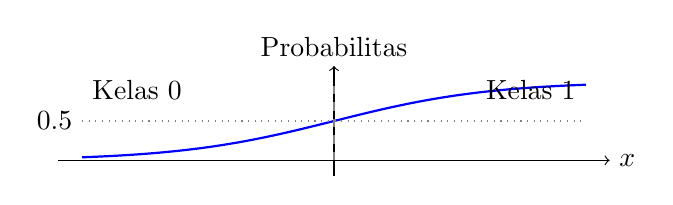
\begin{tikzpicture}[scale=1]
		% Axis
		\draw[->] (-3.5,0) -- (3.5,0) node[right] {$x$};
		\draw[->] (0,-0.2) -- (0,1.2) node[above] {Probabilitas};
		
		% Sigmoid curve
		\draw[thick, domain=-3.2:3.2, samples=100, smooth, variable=\x, blue]
		plot ({\x}, {1/(1 + exp(-\x))});
		
		% Dotted line at x=0
		\draw[dashed, gray] (0,0) -- (0,1);
		
		% Labels for class separation
		\node at (-2.5,0.9) {Kelas 0};
		\node at (2.5,0.9) {Kelas 1};
		
		% Threshold line
		\draw[dotted, gray] (-3.2,0.5) -- (3.2,0.5);
		\node[left] at (-3.2,0.5) {$0.5$};
		
	\end{tikzpicture}
	\caption{Logistic Regression – kurva S untuk memisahkan dua kelas.}
\end{figure}

\subsection*{3. Decision Tree}

\textbf{Decision Tree} meniru cara manusia mengambil keputusan berdasarkan logika “jika–maka” yang digambarkan dalam bentuk struktur pohon. Setiap cabang mewakili kondisi pada suatu fitur, dan setiap daun (leaf) merupakan prediksi akhir.  
Contoh: untuk mengevaluasi apakah seseorang layak mendapat pinjaman, decision tree dapat memeriksa atribut seperti penghasilan, usia, status pekerjaan, dan histori kredit.  
Keunggulan utamanya adalah transparansi — pengguna bisnis dapat memahami dan menelusuri alasan di balik prediksi model.

\begin{figure}[h]
	\centering
	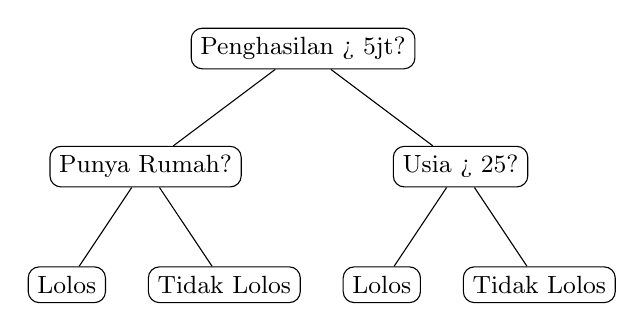
\begin{tikzpicture}[
		level 1/.style={sibling distance=40mm},
		level 2/.style={sibling distance=20mm},
		level distance=15mm,
		every node/.style={draw, rectangle, rounded corners, align=center, font=\small}
		]
		
		\node {Penghasilan > 5jt?}
		child {node {Punya Rumah?}
			child {node {Lolos}}
			child {node {Tidak Lolos}}
		}
		child {node {Usia > 25?}
			child {node {Lolos}}
			child {node {Tidak Lolos}}
		};
		
	\end{tikzpicture}
	\caption{Contoh struktur Decision Tree sederhana untuk evaluasi kelayakan pinjaman.}
\end{figure}

\subsection*{4. K-Nearest Neighbours (K-NN)}

\textbf{K-Nearest Neighbours (K-NN)} bekerja dengan membandingkan data baru dengan data historis yang paling mirip (berdekatan secara “jarak”).  
Model ini tidak membangun fungsi atau pohon, tapi menyimpan semua data historis dan membuat prediksi berdasarkan mayoritas “tetangga terdekat”.  
Contoh: jika ingin mengklasifikasikan tipe pelanggan baru, K-NN akan melihat siapa pelanggan lama yang mirip dari sisi profil dan perilaku, kemudian mengikuti kelompok mayoritas.

\begin{figure}[h]
	\centering
	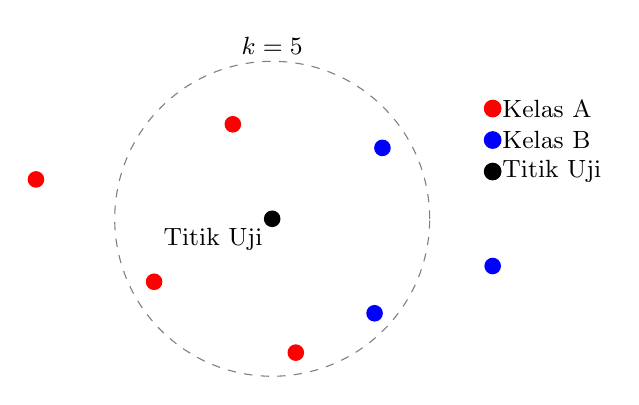
\begin{tikzpicture}[scale=1, every node/.style={font=\small}]
		
		% Titik uji (query point)
		\fill[black] (0,0) circle (3pt);
		\node[below left] at (0,0) {Titik Uji};
		
		% Lingkaran tetangga terdekat (misalnya radius k=5)
		\draw[gray, dashed] (0,0) circle (2);
		
		% Titik-titik kelas merah
		\fill[red] (-0.5, 1.2) circle (3pt);
		\fill[red] (-1.5, -0.8) circle (3pt);
		\fill[red] (0.3, -1.7) circle (3pt);
		
		% Titik-titik kelas biru
		\fill[blue] (1.4, 0.9) circle (3pt);
		\fill[blue] (1.3, -1.2) circle (3pt);
		
		% Titik luar radius (tidak dihitung)
		\fill[red] (-3, 0.5) circle (3pt);
		\fill[blue] (2.8, -0.6) circle (3pt);
		
		% Legenda
		\draw[red, fill=red] (2.8,1.4) circle (3pt);
		\node[right] at (2.8,1.4) {Kelas A};
		
		\draw[blue, fill=blue] (2.8,1.0) circle (3pt);
		\node[right] at (2.8,1.0) {Kelas B};
		
		\draw[black, fill=black] (2.8,0.6) circle (3pt);
		\node[right] at (2.8,0.6) {Titik Uji};
		
		% Label radius k
		\node at (0,2.2) {$k = 5$};
		
	\end{tikzpicture}
	\caption{K-NN – prediksi berdasarkan mayoritas kategori dari 5 tetangga terdekat.}
\end{figure}

\subsection*{Catatan Tambahan}

Pemilihan algoritma tergantung pada jenis data, tujuan prediksi, serta preferensi interpretabilitas.  
Dalam konteks bisnis, decision tree dan linear/logistic regression sering menjadi pilihan awal karena hasilnya mudah dipahami dan dikomunikasikan kepada manajemen \cite{provost2013data}.


\section{Tahapan Proyek Machine Learning dalam Big Data}

Proyek Machine Learning (ML), khususnya supervised learning, mengikuti alur sistematis yang memastikan model dibangun berdasarkan data yang relevan dan dapat digunakan secara efektif untuk mendukung keputusan bisnis. Dalam konteks Big Data, setiap tahap menghadapi tantangan tersendiri karena volume data yang besar, kecepatan pembaruan data, dan keragaman format sumbernya \cite{chen2012,wamba2017}.

Berikut adalah tahapan umum dalam proyek supervised learning dan bagaimana masing-masing terhubung dengan praktik Big Data for Business:

\subsection*{1. Mengumpulkan Data (Data Collection)}

Langkah awal adalah mengumpulkan data dari berbagai sumber: sistem transaksi, sensor IoT, media sosial, CRM, ERP, dan lainnya. Dalam konteks Big Data, tantangan utama adalah:
\begin{itemize}
	\item Volume data yang besar dan terus bertambah,
	\item Variasi format: terstruktur (CSV, database), semi-terstruktur (JSON, XML), dan tidak terstruktur (teks, gambar, audio),
	\item Sering kali data bersifat real-time atau streaming.
\end{itemize}

Pemanfaatan teknologi Big Data seperti Apache Kafka, NiFi, dan Hadoop HDFS umum digunakan dalam proses ini.

\subsection*{2. Membersihkan dan Menyiapkan Data (Data Preparation)}

Data yang dikumpulkan tidak selalu siap pakai. Proses ini melibatkan:
\begin{itemize}
	\item Menghapus duplikasi dan outlier,
	\item Menangani nilai yang hilang (missing values),
	\item Mengubah format dan skala data (normalisasi),
	\item Encoding variabel kategori menjadi angka,
	\item Memilih fitur (feature selection) yang relevan.
\end{itemize}

Pada tahap ini, kualitas data sangat menentukan kualitas model. Dalam konteks Big Data, pendekatan otomatis seperti pipeline data preparation sangat dibutuhkan untuk efisiensi dan skalabilitas \cite{rahm2000dataquality}.

\subsection*{3. Memilih Algoritma}

Bergantung pada tujuan bisnis dan jenis label:
\begin{itemize}
	\item Klasifikasi: Logistic Regression, Decision Tree, Random Forest, SVM.
	\item Regresi: Linear Regression, Gradient Boosting.
\end{itemize}

Faktor lain yang memengaruhi pilihan algoritma antara lain:
\begin{itemize}
	\item Ukuran dataset,
	\item Kebutuhan interpretabilitas,
	\item Waktu komputasi,
	\item Dukungan sistem operasional untuk model tersebut.
\end{itemize}

\subsection*{4. Melatih Model (Model Training)}

Model dilatih menggunakan data historis yang telah dipisahkan menjadi \texttt{training set}. Model belajar dari pola hubungan antara fitur dan label.  
Dalam skala Big Data, proses pelatihan sering membutuhkan pemrosesan paralel, distribusi data, dan optimalisasi beban kerja.

Tools seperti Apache Spark MLlib, TensorFlow, atau Orange (untuk pendekatan visual) umum digunakan.

\subsection*{5. Mengevaluasi Model (Model Evaluation)}

Model kemudian diuji pada \texttt{testing set} untuk mengevaluasi kemampuannya dalam memprediksi data yang belum pernah dilihat.  
Metrik evaluasi bergantung pada tipe prediksi:
\begin{itemize}
	\item \textbf{Klasifikasi:} akurasi, precision, recall, F1-score, ROC-AUC.
	\item \textbf{Regresi:} MAE (mean absolute error), RMSE (root mean squared error), R\textsuperscript{2} score.
\end{itemize}

Evaluasi dalam konteks bisnis juga mempertimbangkan \textit{nilai ekonomis} dari hasil model, bukan hanya performa statistik semata.

\subsection*{6. Menginterpretasikan Hasil untuk Pengambilan Keputusan}

Tahap akhir, tetapi paling kritikal dalam konteks bisnis. Hasil model harus:
\begin{itemize}
	\item Dipahami oleh pemangku kepentingan non-teknis,
	\item Diintegrasikan ke dalam proses bisnis (misalnya sistem rekomendasi, CRM, atau dashboard operasional),
	\item Disertai analisis risiko dan potensi bias algoritmik.
\end{itemize}

Keterlibatan pengguna bisnis dalam interpretasi hasil model sangat penting agar keputusan yang diambil berbasis data namun tetap mempertimbangkan konteks dan strategi organisasi \cite{provost2013data,davenport2018}.

\bigskip

\noindent
Seluruh tahapan ini sebaiknya dilakukan dalam pendekatan iteratif dan kolaboratif antara tim data dan pemangku kepentingan bisnis. Kerangka seperti CRISP-DM atau Data Value Chain dapat digunakan sebagai panduan metodologis.



\section{Proyek Praktik: Prediksi Churn Pelanggan Menggunakan Orange}

Salah satu cara terbaik untuk memahami konsep supervised learning adalah melalui praktik langsung. Dalam bagian ini, mahasiswa akan mempelajari bagaimana membangun model prediksi churn pelanggan menggunakan perangkat lunak \textbf{Orange}, sebuah alat machine learning berbasis visual yang dirancang agar mudah digunakan bahkan oleh pengguna tanpa latar belakang teknis.

\subsection{Kenapa Menggunakan Orange?}

Orange adalah platform open-source untuk analisis data dan machine learning yang menyediakan pendekatan berbasis \textit{drag-and-drop} melalui antarmuka grafis. Tidak seperti banyak framework machine learning lain yang memerlukan pengetahuan pemrograman (seperti Python atau R), Orange memungkinkan pengguna membangun alur analisis (workflow) secara visual dengan menghubungkan blok-blok (widgets) seperti membaca data, memvisualisasi, melatih model, dan mengevaluasi performa.

Beberapa alasan utama mengapa Orange sangat cocok untuk mahasiswa non-IT dalam konteks bisnis dan manajemen:
\begin{itemize}
	\item \textbf{Tanpa Koding:} Semua proses dilakukan melalui antarmuka grafis, sehingga pengguna dapat fokus memahami konsep, bukan sintaks.
	\item \textbf{Pendekatan Modular:} Setiap tahap machine learning—mulai dari preprocessing, training, hingga evaluasi—tersusun dalam blok yang dapat dihubungkan secara fleksibel.
	\item \textbf{Visualisasi yang Kuat:} Orange mendukung berbagai visualisasi seperti scatter plot, confusion matrix, ROC curve, dan decision tree, yang sangat membantu dalam memahami dan menjelaskan hasil model kepada tim manajemen.
	\item \textbf{Cepat untuk Eksplorasi:} Pengguna dapat mencoba berbagai algoritma hanya dengan mengganti blok model, tanpa harus menulis ulang kode.
	\item \textbf{Cocok untuk Pembelajaran Terapan:} Orange sudah banyak digunakan dalam konteks pendidikan, khususnya untuk menjembatani teori machine learning dengan aplikasi praktis di dunia nyata.
\end{itemize}

Dengan menggunakan Orange, mahasiswa diharapkan tidak hanya memahami bagaimana supervised learning bekerja, tetapi juga dapat mengaplikasikannya langsung untuk menjawab tantangan bisnis seperti churn analysis secara intuitif dan kolaboratif, tanpa ha

\subsection{Persiapan dan Instalasi}

Sebelum memulai proyek prediksi churn pelanggan menggunakan Orange, langkah pertama adalah menyiapkan perangkat lunak dan memahami antarmuka utamanya. Orange dapat diinstal dengan mudah di sistem operasi Windows, macOS, maupun Linux tanpa memerlukan keahlian teknis.

\subsubsection*{Langkah 1: Unduh dan Instal Orange}

Orange dapat diunduh secara gratis melalui situs resminya:

\begin{itemize}
	\item \url{https://orangedatamining.com/download}
\end{itemize}

Pilih versi instalasi sesuai sistem operasi Anda:
\begin{itemize}
	\item Untuk pengguna \textbf{Windows}, cukup unduh dan jalankan \texttt{.exe} installer.
	\item Untuk pengguna \textbf{macOS}, unduh file \texttt{.dmg} dan seret ikon Orange ke folder \texttt{Applications}.
	\item Untuk pengguna \textbf{Linux}, instalasi dapat dilakukan melalui \texttt{pip} atau \texttt{conda}, namun disarankan menggunakan installer resmi atau versi portable (AppImage) untuk pemula.
\end{itemize}

Setelah instalasi selesai, jalankan aplikasi Orange dengan mengklik ikonnya di desktop atau di folder aplikasi Anda.

\subsubsection*{Langkah 2: Mengenal Antarmuka Utama Orange}

Setelah Orange terbuka, Anda akan melihat tampilan antarmuka grafis yang sederhana dan intuitif, terdiri dari beberapa komponen utama:

\begin{itemize}
	\item \textbf{Canvas Area:} Ruang kerja utama di mana pengguna menyusun alur (workflow) analisis dengan menghubungkan blok-blok (widgets).
	\item \textbf{Widget Toolbox (di sebelah kiri):} Daftar kategori seperti \texttt{Data}, \texttt{Visualize}, \texttt{Model}, \texttt{Evaluate}, yang masing-masing berisi blok yang dapat digunakan untuk memuat data, menampilkan grafik, membangun model, dan menguji performa.
	\item \textbf{Menu dan Toolbar (atas):} Untuk menyimpan dan membuka workflow, mengatur preferensi, atau mengakses add-on.
	\item \textbf{Output Panels (popup):} Muncul ketika Anda membuka masing-masing widget, berisi konfigurasi dan hasil dari blok tersebut.
\end{itemize}

Setiap widget (misalnya \texttt{File}, \texttt{Scatter Plot}, \texttt{Logistic Regression}) cukup ditarik (drag) ke canvas dan dihubungkan dengan widget lain untuk membentuk alur kerja analisis.

\subsubsection*{Catatan Penting}

Orange secara default sudah menyediakan banyak widget yang cukup untuk supervised learning. Namun, jika diperlukan, Anda juga bisa menambahkan add-on seperti \texttt{Text Mining}, \texttt{Geo}, atau \texttt{Time Series} melalui menu \texttt{Options > Add-ons}.

Dengan perangkat lunak yang sudah siap dan antarmuka yang mudah dipahami, mahasiswa dapat langsung memulai eksperimen membangun model prediksi churn pelanggan secara interaktif dan visual.

\subsection{Deskripsi Dataset}

Untuk proyek praktik ini, kita akan menggunakan \textbf{Telco Customer Churn Dataset}, sebuah dataset yang populer digunakan dalam pembelajaran prediktif untuk mengetahui apakah pelanggan akan berhenti menggunakan layanan (churn) atau tidak. Dataset ini disediakan dalam format CSV dan dapat diunduh dari berbagai sumber publik, termasuk Kaggle:

\begin{itemize}
	\item \url{https://www.kaggle.com/datasets/blastchar/telco-customer-churn}
\end{itemize}

Dataset ini berisi data pelanggan dari sebuah perusahaan layanan telekomunikasi fiktif, mencakup atribut demografis, data kontrak layanan, serta status keaktifan pelanggan.

\subsubsection*{Tujuan Prediksi (Label)}

Kolom target atau label yang ingin diprediksi adalah:
\begin{itemize}
	\item \texttt{Churn}: Menunjukkan apakah pelanggan berhenti menggunakan layanan (\texttt{Yes}) atau tidak (\texttt{No}).
\end{itemize}

Ini merupakan tugas \textbf{klasifikasi biner}, karena hanya ada dua kemungkinan output.

\subsubsection*{Fitur Utama (Input)}

Beberapa fitur penting (atribut input) yang dapat digunakan untuk membangun model prediksi antara lain:

\begin{itemize}
	\item \texttt{gender}: Jenis kelamin pelanggan (Male / Female).
	\item \texttt{SeniorCitizen}: Apakah pelanggan berusia lanjut (0 = Tidak, 1 = Ya).
	\item \texttt{Partner}: Apakah pelanggan memiliki pasangan.
	\item \texttt{Dependents}: Apakah pelanggan memiliki tanggungan keluarga.
	\item \texttt{tenure}: Lama pelanggan menggunakan layanan (dalam bulan).
	\item \texttt{PhoneService}: Apakah pelanggan menggunakan layanan telepon.
	\item \texttt{MultipleLines}: Apakah pelanggan memiliki lebih dari satu saluran.
	\item \texttt{InternetService}: Jenis layanan internet (DSL, Fiber optic, atau No).
	\item \texttt{OnlineSecurity}, \texttt{OnlineBackup}, \texttt{TechSupport}: Status layanan tambahan.
	\item \texttt{Contract}: Tipe kontrak (Month-to-month, One year, Two year).
	\item \texttt{PaperlessBilling}: Apakah menggunakan tagihan digital.
	\item \texttt{PaymentMethod}: Metode pembayaran (Credit card, Bank transfer, dsb).
	\item \texttt{MonthlyCharges}, \texttt{TotalCharges}: Jumlah biaya bulanan dan total biaya.
\end{itemize}

\subsubsection*{Catatan Pengolahan Data}

Sebelum digunakan dalam Orange, pastikan dataset dalam format CSV telah:
\begin{itemize}
	\item Memiliki nilai yang lengkap (tidak kosong) pada kolom penting seperti \texttt{Churn}, \texttt{tenure}, dan \texttt{MonthlyCharges}.
	\item Memiliki tipe data yang tepat — misalnya \texttt{TotalCharges} terkadang terbaca sebagai teks, perlu dikonversi menjadi angka.
	\item Menggunakan label target \texttt{Churn} dalam format kategorikal (Yes/No) yang dikenali Orange sebagai variabel kelas.
\end{itemize}

Dataset ini mencerminkan situasi nyata yang umum dihadapi perusahaan telekomunikasi dan menyediakan konteks yang kuat bagi mahasiswa bisnis untuk memahami bagaimana machine learning dapat dimanfaatkan untuk retensi pelanggan.

 
 
\subsection{Langkah-Langkah Workflow}

Berikut adalah alur kerja (\textit{workflow}) langkah demi langkah yang dapat diikuti di Orange untuk membangun model prediksi churn pelanggan. Seluruh proses ini dilakukan secara visual, tanpa pemrograman, hanya dengan menghubungkan blok-blok (widget) di dalam canvas.

\subsubsection*{1. Memuat Dataset dari File CSV}

Gunakan widget \texttt{File} untuk memuat dataset \texttt{Telco-Customer-Churn.csv}. Pastikan:
\begin{itemize}
	\item Format file adalah CSV.
	\item Kolom \texttt{Churn} diatur sebagai \texttt{Target} (label) oleh Orange secara otomatis, atau atur secara manual via \texttt{Select Columns}.
\end{itemize}

\textbf{Langkah:} Tambahkan widget \texttt{File} $\rightarrow$ Klik dua kali $\rightarrow$ Pilih file dataset.

\subsubsection*{2. Eksplorasi Visualisasi Awal}

Tambahkan widget \texttt{Box Plot} dan \texttt{Scatter Plot} untuk memahami distribusi data dan hubungan antar variabel.

Contoh eksplorasi:
\begin{itemize}
	\item Box plot: Lihat distribusi \texttt{MonthlyCharges} berdasarkan status \texttt{Churn}.
	\item Scatter plot: Amati hubungan antara \texttt{tenure} dan \texttt{TotalCharges}.
\end{itemize}

\textbf{Langkah:} Hubungkan \texttt{File} $\rightarrow$ \texttt{Box Plot} / \texttt{Scatter Plot}.

\subsubsection*{3. Seleksi Atribut dan Prapemrosesan}

Gunakan widget \texttt{Select Columns} untuk memilih fitur yang relevan dan membuang kolom tidak informatif (misalnya \texttt{customerID}).  
Gunakan \texttt{Continuize} untuk mengubah variabel numerik jika dibutuhkan oleh algoritma.

\textbf{Langkah:} Tambahkan \texttt{Select Columns} setelah \texttt{File}, lalu tentukan fitur yang akan digunakan dan label target.

\subsubsection*{4. Split Data menjadi Training dan Testing}

Gunakan widget \texttt{Data Sampler} untuk membagi data menjadi dua bagian:
\begin{itemize}
	\item 70\% untuk \texttt{Training set},
	\item 30\% untuk \texttt{Testing set}.
\end{itemize}

\textbf{Langkah:} Tambahkan \texttt{Data Sampler} $\rightarrow$ atur \texttt{Proportion = 0.7} $\rightarrow$ output: \texttt{Data} dan \texttt{Remaining Data}.

\subsubsection*{5. Pilih Algoritma: Decision Tree atau Logistic Regression}

Tambahkan salah satu model berikut:
\begin{itemize}
	\item \texttt{Logistic Regression}: cocok untuk klasifikasi churn dengan output probabilistik.
	\item \texttt{Tree}: cocok untuk interpretasi visual dan pembentukan aturan.
\end{itemize}

\textbf{Langkah:} Hubungkan \texttt{Training set} dari \texttt{Data Sampler} ke model pilihan.

\subsubsection*{6. Evaluasi Hasil: Akurasi dan Confusion Matrix}

Tambahkan widget \texttt{Test and Score} untuk mengevaluasi model menggunakan data testing.  
Lanjutkan dengan \texttt{Confusion Matrix} untuk melihat distribusi prediksi benar dan salah.

\begin{itemize}
	\item Metrik utama: Accuracy, Precision, Recall, AUC.
	\item Confusion Matrix: Prediksi vs Realitas (True Positives, False Negatives, dll).
\end{itemize}

\textbf{Langkah:} 
\begin{enumerate}
	\item Hubungkan \texttt{Model} dan \texttt{Testing set} ke \texttt{Test and Score}.
	\item Hubungkan hasil dari \texttt{Test and Score} ke \texttt{Confusion Matrix}.
\end{enumerate}

\subsubsection*{7. Interpretasi Pohon Keputusan dan Fitur Penting}

Jika menggunakan \texttt{Tree}, tambahkan widget \texttt{Tree Viewer} untuk menampilkan struktur pohon. Ini sangat bermanfaat bagi pengguna bisnis karena menunjukkan logika prediksi secara eksplisit.

Hal-hal yang dapat dianalisis:
\begin{itemize}
	\item Jalur keputusan: misalnya, pelanggan dengan \texttt{tenure < 5 bulan} dan \texttt{MonthlyCharges > 70} cenderung churn.
	\item Fitur yang paling sering muncul di cabang atas biasanya adalah fitur paling penting.
\end{itemize}

\textbf{Langkah:} Hubungkan \texttt{Tree} $\rightarrow$ \texttt{Tree Viewer}.

\bigskip

\noindent
Dengan menyelesaikan workflow ini, mahasiswa akan memperoleh pengalaman langsung membangun model prediktif, menilai akurasinya, dan menerjemahkan hasilnya ke dalam wawasan yang berguna untuk pengambilan keputusan bisnis.

\subsection{Interpretasi Bisnis}

Setelah model machine learning dibangun dan dievaluasi, tahap berikutnya yang sangat penting adalah menginterpretasikan hasilnya dalam konteks bisnis. Tujuan utama dari prediksi churn bukan hanya mengetahui siapa yang kemungkinan besar akan berhenti berlangganan, tetapi bagaimana informasi tersebut dapat digunakan untuk mengambil keputusan yang tepat.

\subsubsection*{Makna Hasil Model}

Hasil dari model supervised learning, seperti Logistic Regression atau Decision Tree, memberikan dua hal utama:
\begin{itemize}
	\item \textbf{Prediksi churn untuk setiap pelanggan:} apakah pelanggan diperkirakan akan churn (\texttt{Yes}) atau tidak (\texttt{No}).
	\item \textbf{Probabilitas atau skor keyakinan model:} seberapa besar kemungkinan seorang pelanggan akan churn.
\end{itemize}

Model juga memberikan wawasan tentang fitur-fitur apa yang paling berpengaruh terhadap keputusan model, seperti:
\begin{itemize}
	\item Pelanggan dengan \texttt{tenure} (lama berlangganan) rendah lebih rentan churn.
	\item Pelanggan dengan \texttt{MonthlyCharges} tinggi dan kontrak bulanan lebih sering churn dibandingkan mereka yang menggunakan kontrak jangka panjang.
	\item Layanan seperti \texttt{OnlineSecurity} atau \texttt{TechSupport} dapat menjadi faktor retensi yang signifikan.
\end{itemize}

\subsubsection*{Keputusan Strategis yang Dapat Diambil}

Dengan informasi tersebut, perusahaan dapat mengembangkan strategi retensi pelanggan yang lebih tepat sasaran, antara lain:

\begin{itemize}
	\item \textbf{Segmentasi Intervensi:} Fokuskan program retensi hanya pada pelanggan yang diprediksi akan churn, sehingga penggunaan anggaran lebih efisien.
	\item \textbf{Personalisasi Penawaran:} Berikan insentif khusus (diskon, bonus layanan, upgrade) kepada pelanggan berisiko tinggi, terutama mereka yang memiliki potensi nilai jangka panjang.
	\item \textbf{Perbaikan Layanan:} Jika banyak pelanggan churn karena faktor tertentu (misalnya tidak menggunakan layanan tambahan), maka perusahaan dapat melakukan edukasi atau bundling layanan.
	\item \textbf{Desain Kontrak:} Model dapat membantu menentukan struktur kontrak yang lebih mengikat namun tetap menarik bagi pelanggan baru dan eksisting.
\end{itemize}

\subsubsection*{Dampak bagi Pengambilan Keputusan}

Interpretasi hasil model secara tepat memungkinkan perusahaan:
\begin{itemize}
	\item Mengantisipasi churn secara proaktif, bukan reaktif.
	\item Membuat keputusan berdasarkan data, bukan hanya intuisi.
	\item Meningkatkan ROI dari program loyalitas dan kampanye retensi.
	\item Memperkuat pemahaman tentang perilaku pelanggan berdasarkan pola data historis.
\end{itemize}

Dengan demikian, model machine learning bukan sekadar alat teknis, tetapi menjadi \textbf{sumber wawasan strategis} yang mendukung manajemen dalam menciptakan pengalaman pelanggan yang lebih baik dan memperpanjang siklus hidup pelanggan secara berkelanjutan.


\section{Evaluasi Model dan Ukuran Kinerja}

Evaluasi model merupakan tahap krusial dalam supervised learning karena membantu menentukan apakah model yang dibangun mampu memberikan prediksi yang akurat dan bermanfaat dalam konteks bisnis. Dalam kasus prediksi churn pelanggan, kesalahan dalam memprediksi siapa yang akan berhenti dapat berdampak langsung terhadap strategi retensi dan efisiensi biaya.

Beberapa ukuran kinerja utama yang umum digunakan adalah sebagai berikut:

\subsection*{1. Akurasi (Accuracy)}

Akurasi menunjukkan seberapa besar proporsi prediksi model yang benar dibandingkan dengan seluruh data. Misalnya, jika dari 100 pelanggan model berhasil memprediksi 85 dengan benar (baik churn maupun tidak churn), maka akurasinya adalah 85\%.

\textbf{Kelebihan:} Mudah dipahami dan dihitung.  
\textbf{Kekurangan:} Tidak selalu mencerminkan performa sebenarnya, terutama jika data tidak seimbang (misalnya 90\% pelanggan tidak churn).

\subsection*{2. Precision}

Precision mengukur dari seluruh prediksi churn, berapa banyak yang benar-benar churn.  
\[
\text{Precision} = \frac{\text{True Positives}}{\text{True Positives + False Positives}}
\]

\textbf{Contoh:} Jika model memprediksi 40 pelanggan akan churn, tetapi hanya 30 yang benar-benar churn, maka precision = 75\%.

\textbf{Konteks bisnis:} Precision penting ketika biaya mengintervensi pelanggan yang sebenarnya tidak akan churn cukup tinggi (misalnya diskon atau insentif yang sia-sia).

\subsection*{3. Recall (Sensitivity)}

Recall mengukur dari seluruh pelanggan yang benar-benar churn, berapa yang berhasil diprediksi oleh model.

\[
\text{Recall} = \frac{\text{True Positives}}{\text{True Positives + False Negatives}}
\]

\textbf{Contoh:} Jika ada 50 pelanggan yang benar-benar churn, dan model hanya berhasil mendeteksi 30, maka recall = 60\%.

\textbf{Konteks bisnis:} Recall penting jika perusahaan ingin meminimalkan jumlah pelanggan yang hilang tanpa intervensi.

\subsection*{4. F1-Score}

F1-score adalah harmonisasi antara precision dan recall. Cocok digunakan ketika kita ingin menyeimbangkan antara kesalahan prediksi positif palsu (false positives) dan negatif palsu (false negatives).

\[
\text{F1-Score} = 2 \times \frac{\text{Precision} \times \text{Recall}}{\text{Precision} + \text{Recall}}
\]

\textbf{Konteks bisnis:} F1-score sangat berguna saat data tidak seimbang atau saat kita tidak hanya fokus pada satu metrik.

\subsection*{Memilih Metrik yang Sesuai dengan Tujuan Bisnis}

Dalam dunia nyata, tidak ada satu metrik yang “terbaik” untuk semua situasi. Pemilihan metrik harus disesuaikan dengan tujuan bisnis:

\begin{itemize}
	\item Jika \textbf{biaya kehilangan pelanggan sangat tinggi}, maka recall menjadi prioritas (lebih baik memprediksi lebih banyak kemungkinan churn, meskipun ada beberapa false positives).
	\item Jika \textbf{biaya intervensi mahal} (misalnya memberikan diskon), precision lebih penting agar intervensi hanya dilakukan pada pelanggan yang benar-benar berisiko.
	\item Jika kedua biaya sama penting, gunakan F1-score untuk menyeimbangkan keduanya.
\end{itemize}

Sebagai bagian dari proses evaluasi, Orange menyediakan metrik ini secara otomatis melalui widget \texttt{Test \& Score} dan visualisasi melalui \texttt{Confusion Matrix}. Hal ini memudahkan pengguna non-teknis untuk memahami performa model dan menentukan langkah strategis berdasarkan hasil evaluasi tersebut.




\section{Rangkuman}

Machine Learning (ML), khususnya pendekatan supervised learning, merupakan tahap lanjutan dalam strategi Big Data yang berfokus pada penciptaan nilai melalui analitik prediktif dan preskriptif. Setelah data dikumpulkan, disimpan, dan diproses, ML memungkinkan organisasi tidak hanya memahami apa yang terjadi di masa lalu (descriptive analytics), tetapi juga memprediksi apa yang akan terjadi dan merekomendasikan tindakan terbaik yang dapat diambil (prescriptive analytics) \cite{provost2013data}. Dalam konteks bisnis, ML menjadi enabler utama bagi pengambilan keputusan berbasis data, yang lebih cepat, akurat, dan relevan terhadap kondisi pasar yang dinamis.

Ke depan, organisasi dapat mengeksplorasi pendekatan lanjutan seperti AutoML (automated machine learning) untuk menyederhanakan proses pemodelan, serta mengintegrasikan hasil ML ke dalam dashboard interaktif yang mudah diinterpretasi oleh manajemen. Visualisasi hasil prediksi, pelacakan kinerja model, dan pembaruan model berbasis data baru merupakan aspek penting dalam integrasi ML dengan sistem pengambilan keputusan sehari-hari. Dengan membangun budaya data-driven dan tata kelola data yang kuat, Machine Learning dapat dioptimalkan sebagai aset strategis dalam keseluruhan arsitektur Big Data for Business.
